
%set ukuran paper jadi a4 sama 12 pixel font
\documentclass[a4paper,12pt, bahasa]{article}
\usepackage{graphicx} % Required for inserting images

%hyprlink desuwa
\usepackage{hyperref}
\hypersetup{
    colorlinks,
    citecolor=black,
    filecolor=black,
    linkcolor=blue,
    urlcolor=blue
}
%ganti jadi roman
\usepackage{times}

%set margin
\usepackage{geometry}
\geometry{margin=2cm}

%float
\usepackage{float}

%set bahasa indonesia
\usepackage[indonesian]{babel}
\captionsbahasa


\usepackage[backend=biber, style=alphabetic, sorting=none]{biblatex}
\addbibresource{ref.bib}

%set spacing 1.5
\usepackage{setspace}
\onehalfspacing{}
\usepackage{tocloft}

%bikin tabel berwarna
\usepackage[table,xcdraw]{xcolor}
\renewcommand{\cftpartleader}{\cftdotfill{\cftdotsep}}

%bikin judul utama centering
% \usepackage{titlesec}
% \titleformat{\section}[hang]{\normalfont\Large\bfseries}{\thesection}{1em}{\centering}
%idk harus pake date biar gak nongol di title
\date{}

%judul dokumen
\title{Laporan Installasi ChatGPT di PC atau notebook}

\begin{document}
  

\maketitle
\begin{figure}[ht]
  \begin{center}
    
\includegraphics[width=0.5\textwidth]{images/logo.png}
  \end{center}
\end{figure}
\vspace{1 cm}
\thispagestyle{empty}

\begin{center}
    \begin{tabular}{ll}
         Mata Kuliah& Kecerdasan Buatan\\
         Dosen Pengampu& Uro Abdul Rohim, M.T \\
    \end{tabular}\\
    \vspace{0.5cm}
    Disusun Oleh: \\
    \begin{tabular}{ll}
         1.& Rifqi Fadil Fahrial (1222646)\\
         2.& Firli Nur Rizki (1223601)\\
    \end{tabular}\\
    \vspace{3cm}

  \textbf {TEKNIK INFORMATIKA} \\
  \textbf {FAKULTAS INFORMATIKA} \\
  \textbf {STMIK BANDUNG} \\
  \textbf {2024} \linebreak
\end{center}
\pagebreak
\section*{Abstrak}
\setcounter{page}{1}
\addcontentsline{toc}{section}{\protect\numberline{}LEMBAR PENGESAHAN KOORDINATOR}
Penelitian ini berfokus pada implementasi Large Language Model (LLM) menggunakan
framework Olama. LLM telah menjadi kunci dalam perkembangan Natural Language
Processing (NLP), dan Olama menawarkan kemudahan dalam instalasi serta penggunaan
model ini. Makalah ini akan memaparkan langkah-langkah teknis instalasi, pengujian, serta
hasil dari eksperimen implementasi LLM pada Olama. Hasilnya menunjukkan bahwa Olama
mampu menyederhanakan proses instalasi dengan performa yang memadai. Beberapa
tantangan yang dihadapi akan didiskusikan, dan penelitian ini diakhiri dengan analisis
performa serta kesimpulan terkait efektivitas Olama dalam penerapan LLM.

\section*{Kata Kunci}
\addcontentsline{toc}{section}{\protect\numberline{}LEMBAR PENGESAHAN KOORDINATOR}
\textit{LLM, Olama, Instalasi, AI, Deep Learning, NLP}

\section{Pendahuluan}
\subsection{Latar Belakang}
Large Language Models (LLM) seperti GPT-3 dan GPT-NeoX membutuhkan sumber daya
komputasi yang besar untuk dijalankan, biasanya di cloud. Namun, dengan menggunakan
OLaMA (Open Language Model for All), model tersebut dapat dijalankan secara lokal di
komputer pribadi, memberikan kontrol lebih terhadap privasi dan data. Eksperimen ini
bertujuan untuk menginstal OLaMA di Linux dan menjalankan LLM secara lokal tanpa koneksi
internet.
Dalam eksperimen ini, kami mencoba menginstal Large Language Model (LLM) secara lokal
menggunakan OLAMA sebagai platform untuk mempercepat proses pengolahan LLM.
Eksperimen ini bertujuan untuk mengevaluasi proses instalasi, kinerja, dan kompatibilitas
OLAMA dengan sistem dan LLM yang digunakan. LLM yang diuji dalam eksperimen ini adalah
model [Nama LLM], yang memiliki kemampuan pemrosesan bahasa yang besar dan sering
digunakan dalam berbagai aplikasi AI. Utamakan laptop / PC kalian

\subsection{Tujuan Eksperimen}
Eksperimen ini bertujuan untuk menjelaskan langkah-langkah teknis dalam menginstal
LLM menggunakan Olama dan mengevaluasi performa serta efisiensinya pada tugas NLP.

\section{Metodologi}
\subsection{Alat dan Bahan}
Eksperimen ini menggunakan sistem operasi Ubuntu 20.04, Python 3.x, serta berbagai
library. Olama juga digunakan sebagai framework utama dalam instalasi dan konfigurasi
LLM. 

\subsection{Tahapan Instalasi}
tahapan instalasi dilakukan dengan urutan sebagai berikut:
\begin{enumerate}
  \item Instalasi Ollama dilakukan dengan menjalankan bash script yang disediakan pada \textit{website} ollama dengan spesifik pada sistem operasi yang dipakai pada perangkat
  \item Konfigurasi LLM dengan mengikuti dokumentasi Ollama untuk model-model yang diperlukan / spesifik
  \item Pengujian model dengan input teks sederhana untuk memastikan fungsi dari LLM berjalan dengan semestinya
\end{enumerate}

\subsection{Pengujian}
Pengujian dilakukan dengan memasukan beberapa input teks ke dalam LLM yang sudah diinstall. Kemudian ditest dengan menggunakan input yang diberikan dan menghasilkan hasil yang sesuai dengan ekpektasi:

\section{Instalasi}

Langkah awal untuk menginstall Ollama adalah dengan mengunjungi situs \url{https://ollama.com/download} kemudian pilihlah sistem operasi yang digunakan pada perangkat, untuk kasus saat ini menggunakan sistem Operasi Linux. 

\begin{figure}[H]
  \begin{center}
    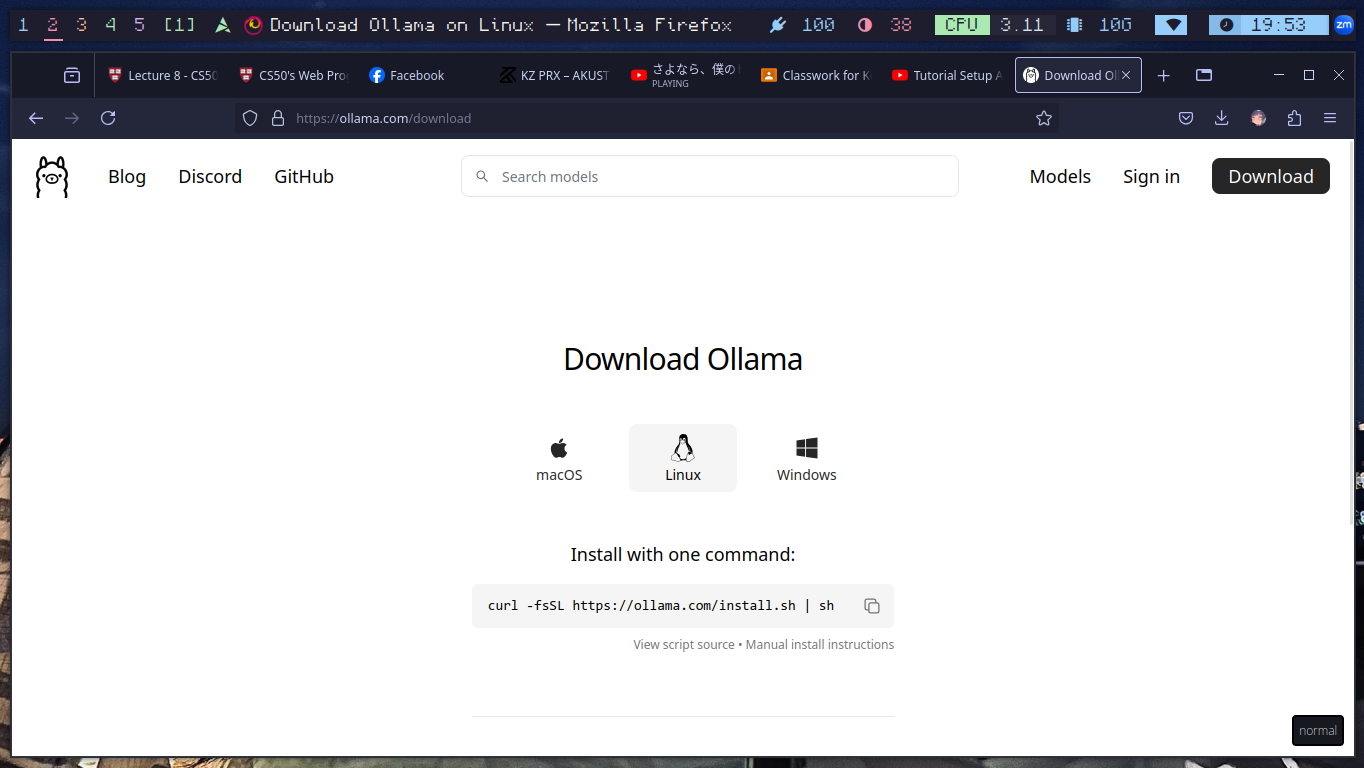
\includegraphics[width=0.80\textwidth]{images/gambar1.png}
    \caption{Tampilan Website Ollama}
  \end{center}
\end{figure}

kemudian akan didapatkan perintah mengenai cara menginstall Ollama di perangkat kemudian ikuti petunjuk yang ditampilkan oleh website, dalam kasus ini hanya perlu menjalankan perintah yang ditampilkan oleh website ke \textit{terminal emulator} untuk menjalankannya. 

\begin{figure}[H]
  \begin{center}
    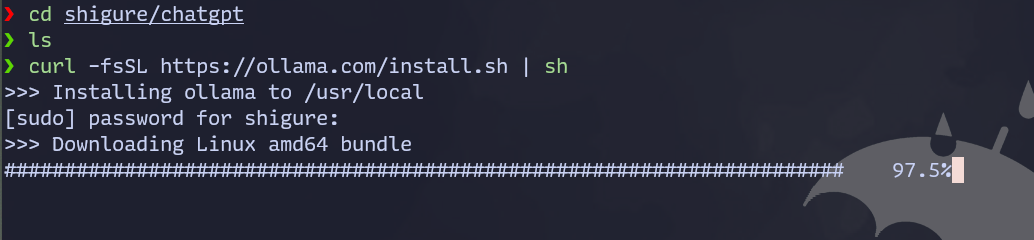
\includegraphics[width=0.80\textwidth]{images/gambar-2.png}
    \caption{Menjalankan Program installasi Ollama}
  \end{center} 
\end{figure}

  kemudian tunggu beberapa saat untuk aplikasi mengunduh depedensi yang diperlukan. 

\begin{figure}[H]
  \begin{center}
    
\includegraphics[width=0.80\textwidth]{images/gambar2.png}
    \caption{Pemasangan Selesai}
  \end{center}
\end{figure}

Setelah selesai menginstall maka dapat dicek apakah aplikasi Ollama ini telah terpasang pada perangkat dengan mengetik "ollama -v" untuk menampilkan versi dari Ollama yang terinstall dan mengecek instalasi. 

\begin{figure}[H]
  \begin{center}
    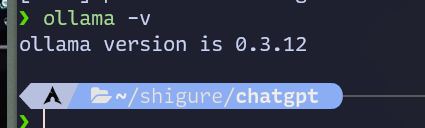
\includegraphics[width=0.80\textwidth]{images/gambar3.png}
    \caption{Verifikasi Installasi Ollama}
  \end{center}
\end{figure}

setelah itu untuk mendapatkan Model dari LLM dapat didapatkan dengan mengetik "Ollama pull {Model yang diinginkan}" untuk kasus ini dipilih "\textit{Deepseek-coder}" dikarenakan Models yang ringan dan cocok untuk perangkat yang digunakan saat ini. 

\begin{figure}[H]
  \begin{center}
    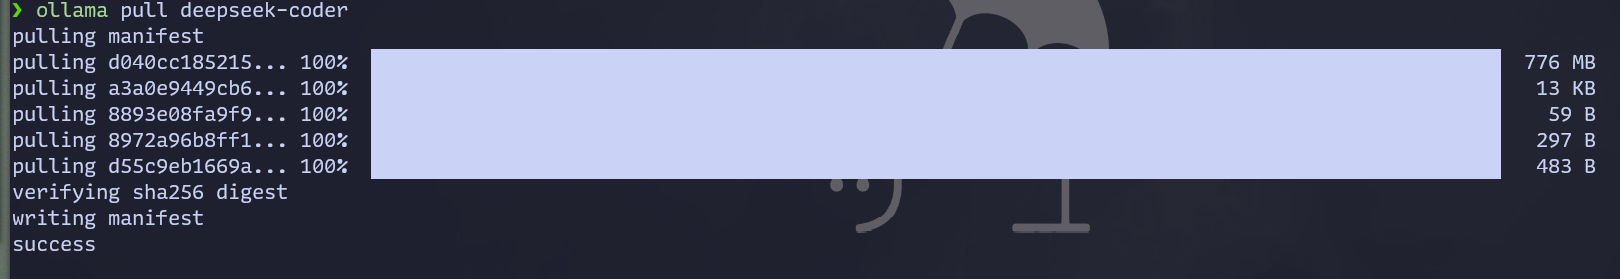
\includegraphics[width=0.80\textwidth]{images/gambar4.png}
    \caption{Pengunduhan Model LLM Deepseek-coder}
  \end{center}
\end{figure}

kemudian untuk menjalankan LLM yang telah diunduh menggunakan Ollama dengan mengetik "Ollama run {Model yang dipilih} Deepseek-coder" kemudian akan masuk tampilan Interpreter yang tinggal memasukan teks berisi pertanyaaan yang kemudian akan dijawab oleh LLM ini, tunggu beberapa saat agar jawabanya selesai.  untuk contohnya bertanya mengenai "How to center an image in html" yang kemudian dijawab dengan contoh code yang ditulis dengan bahasa HTML dan CSS

\begin{figure}[H]
  \begin{center}
    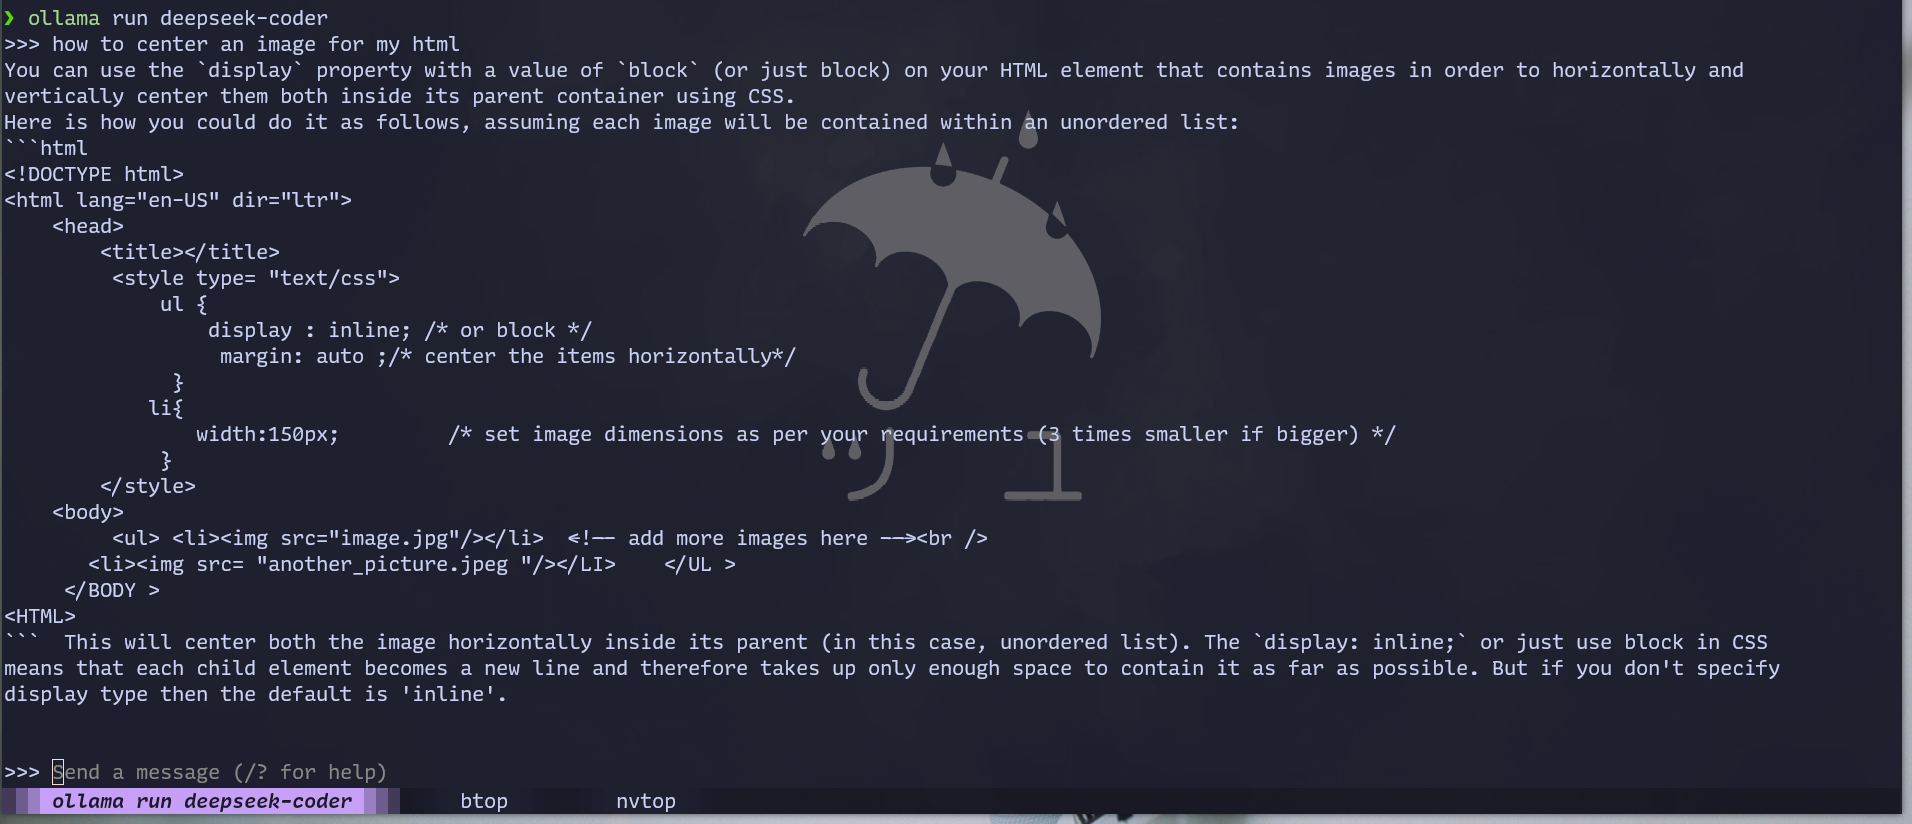
\includegraphics[width=0.80\textwidth]{images/gambar5.png}
    \caption{Hasil LLM Deepseek-coder menggunakan Ollama}
  \end{center}
\end{figure}
Bukti dari jalannya LLM pada perangkat pribadi, pada sistem monitor menunjukkan lonjakan load pada CPU yang tinggi namun tidak ada load pada GPU dikarenakan Model yang digunakan terbilang ringan dan masih belum perlu menggunakan GPU sehingga hanya berfokus pada CPU saja\dots

\begin{figure}[H]
  \begin{center}
    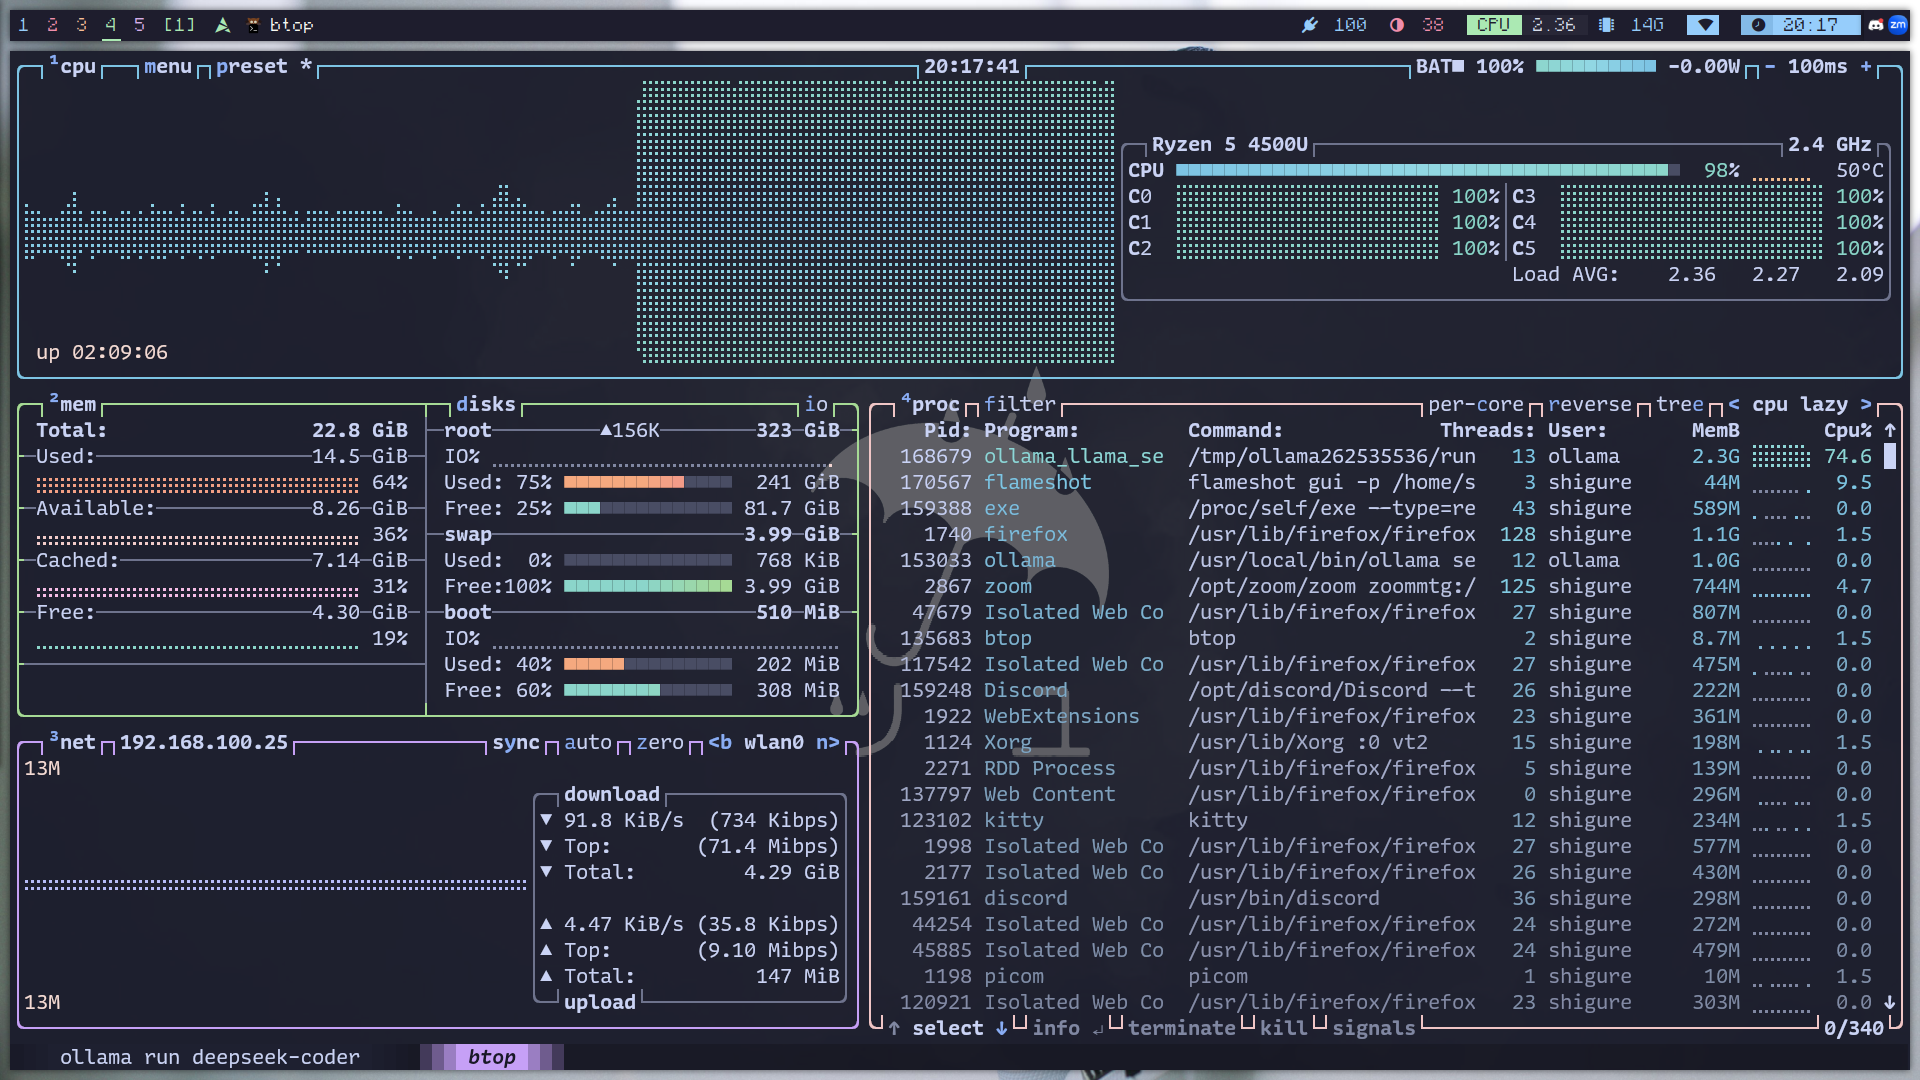
\includegraphics[width=0.80\textwidth]{images/gambar6.png}
    \caption{Sistem monitor CPU menunjukkan beban tinggi}
  \end{center}
\end{figure}
\begin{figure}[H]
  \begin{center}
    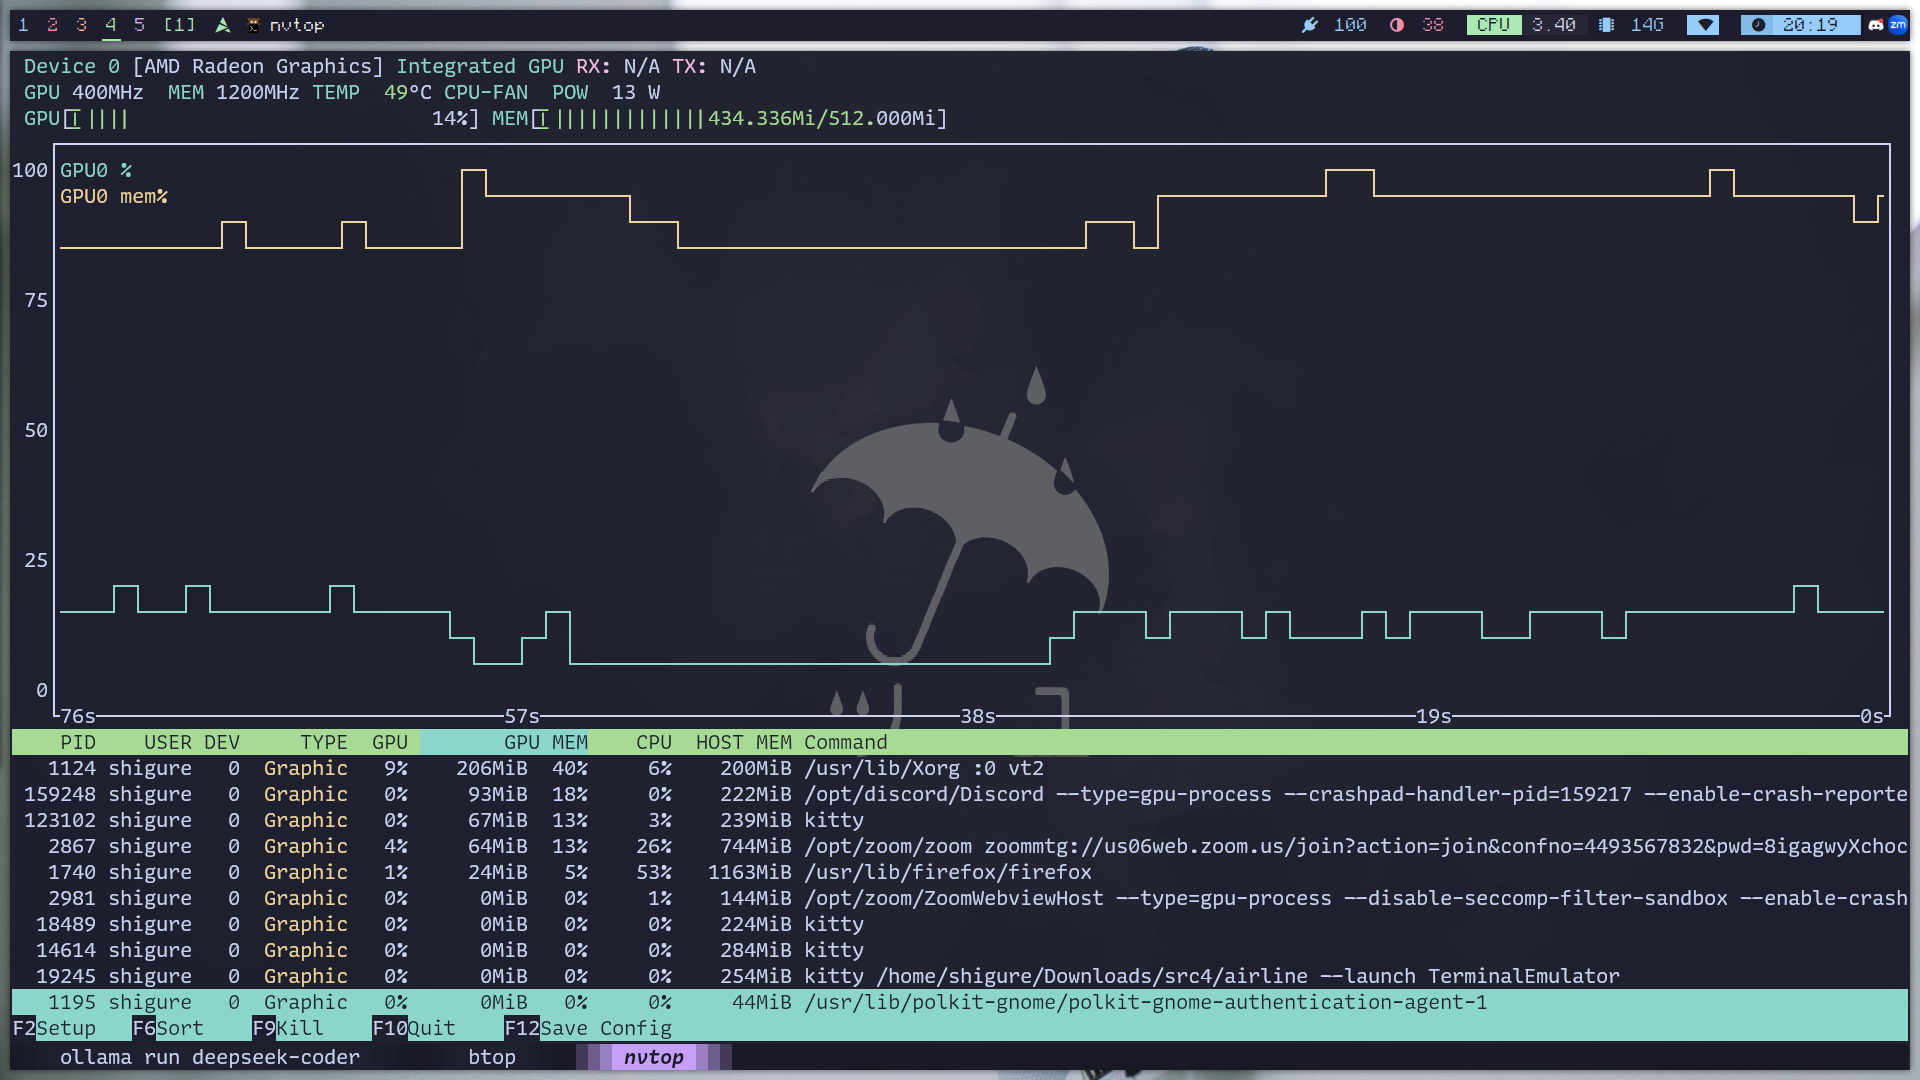
\includegraphics[width=0.80\textwidth]{images/gambar7.png}
    \caption{Sistem monitor GPU tidak menunjukkan beban pada GPU}
  \end{center}
\end{figure}

yang terakhir untuk menampilkan informasi mengenai Model yang digunakan saat ini dapat dengan mudah dengan mengetik "/show info" pada \textit{terminal emulator} kemudian akan tampil informasi mengenai Model yang saat ini sedang digunakan 
\begin{figure}[H]
  \begin{center}
    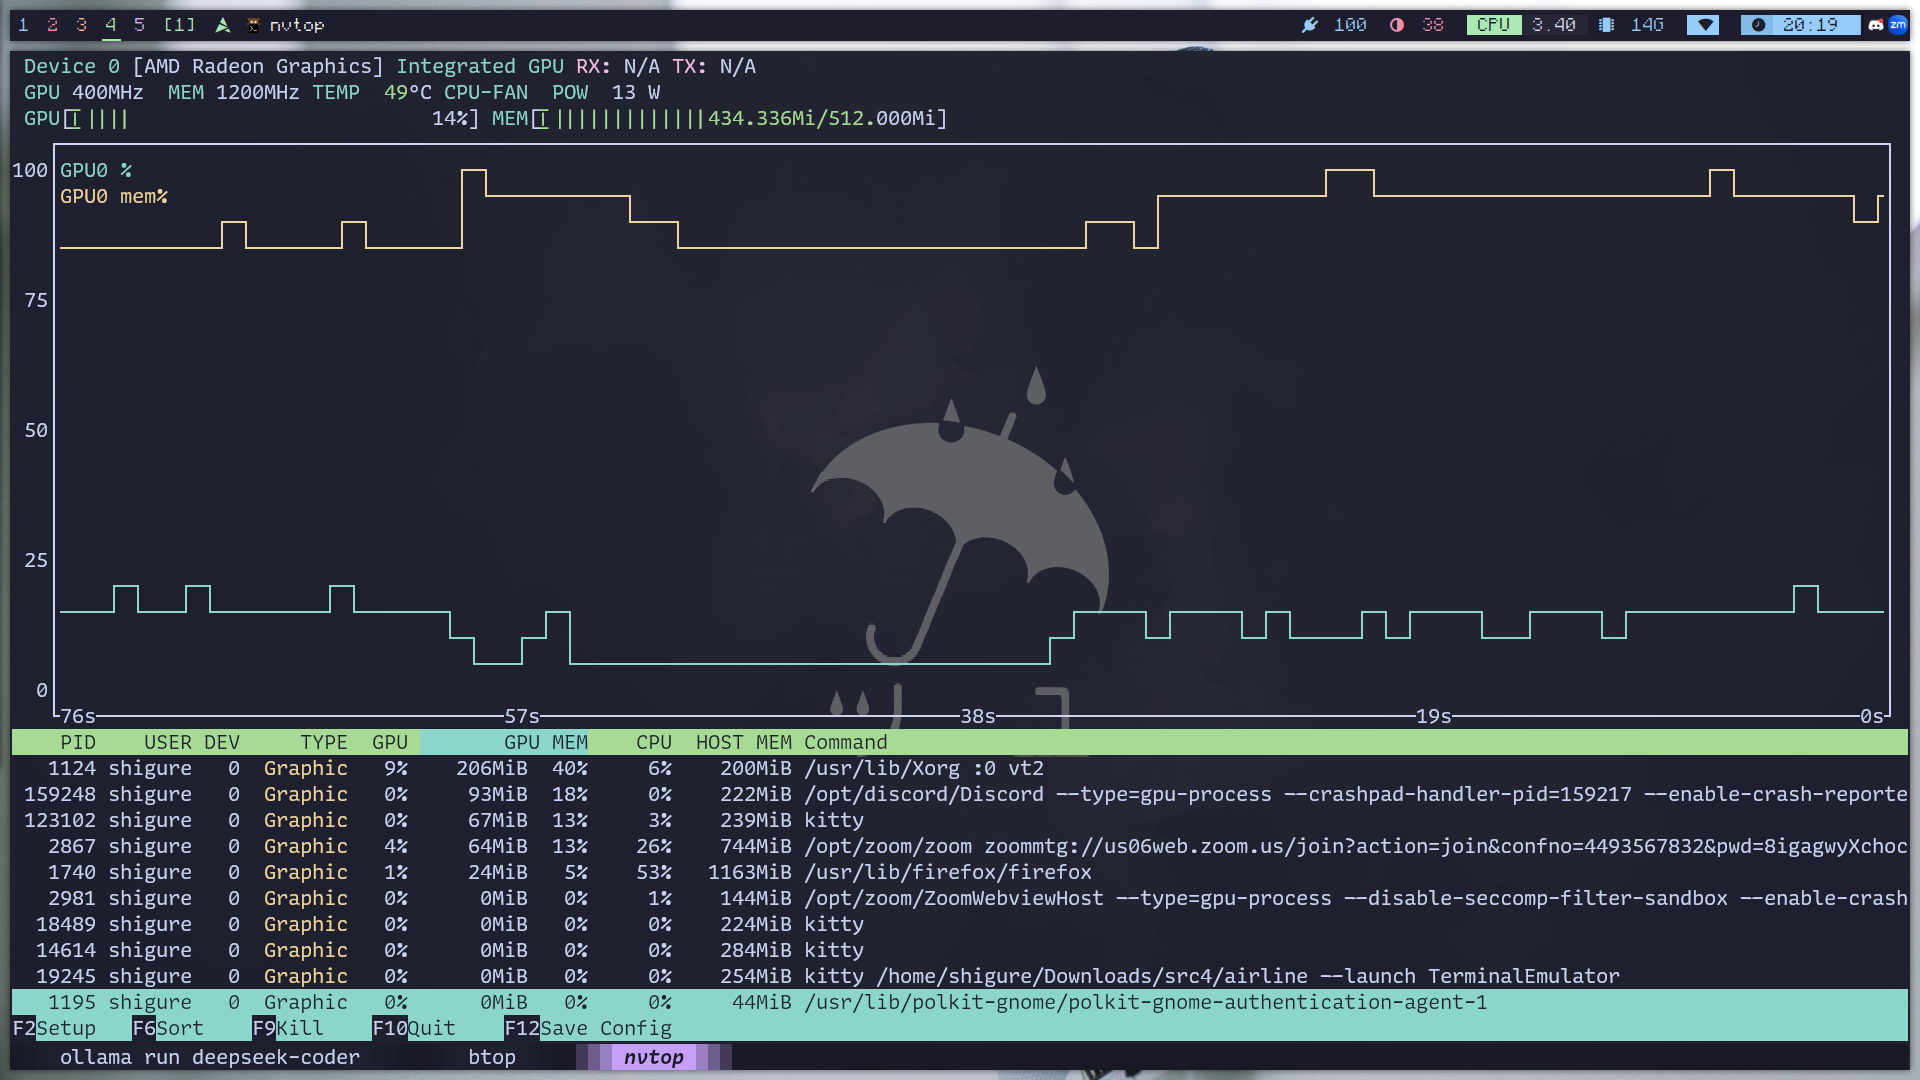
\includegraphics[width=0.80\textwidth]{images/gambar7.png}
    \caption{Informasi mengenai Model yang digunakan}
  \end{center}
\end{figure}

\end{document}
